\documentclass{beamer}
% \usepackage{beamerthemesplit} // Activate for custom appearance
\usepackage{beamerthemesintef}
\usepackage{caption}

\titlebackground*{assets/background}
\title{Point Cloud Occupancy with Dynamic Planes}
\subtitle{Computer Vision Course Project}
\course{Master's Degree in Artificial Intelligence and Robotics}
\author{\href{mailto:bugli.1934824@studenti.uniroma1.it}{Eugenio Bugli}}
\IDnumber{1934824}
\date{Academic Year 2024/2025}

\begin{document}
\maketitle

\section{Introduction}

\begin{frame}{What is the Addressed Problem}
\begin{itemize}
	  \item We would like to learn the \textbf{Occupancy} values of points inside a bounding box
	  \item We learn the features and the dynamic planes 
	  \item During Inference we reconstruct meshes with Multiresolution IsoSurface Extraction
\end{itemize}
\end{frame} 

\section{Dataset}

\begin{frame}{FAUST Dataset}
    This Dataset is composed by high-resolution \textbf{human scans} of 10 different bodies in 30 different poses. 
    \begin{itemize}
    \item Each samples inside the training set is composed by the scan and the registration, while we have only the scan for the test set.
    \item The test set is composed by 200 scans, while the training has 100 scans.
    \item About 80 \% fo the initial training set has been used for training, while the other 20 \% has been used for validation.
    \end{itemize}
\end{frame}


% \begin{frame}{Examples from the Dataset}
%   \begin{columns}[t]
%     \column{0.48\textwidth}
%       \centering
%       \includegraphics[width=\textwidth]{../media/test_scan_137.gif} % first image
%       % \caption{Image 1} % optional: add caption using a note or overlay
%     \column{0.48\textwidth}
%       \centering
%       \includegraphics[width=\textwidth]{../media/test_scan_191.gif} % second image
%       % \caption{Image 2}
%   \end{columns}
% \end{frame}

\begin{frame}{Data Processing}
    Starting from the meshes given by the Dataset, some pre-processing is needed:
    \begin{itemize}
        \item We need to randomly sample \textbf{3000} points from the mesh surface and add a perturbation (Gaussian noise) to them.
        \item We need to randomly sample \textbf{2048} points from the bounding box that contains the original mesh.
    \end{itemize}
    These noisy clouds are then used to learn the features and the geometry of the object through the Encoder, while the other points are used in the decoding part of the network.
\end{frame}

\begin{frame}{Data Augmentation}

  Here is some introductory text explaining the data augmentation process. This text spans the full width of the frame.
  
  \vspace{1em}

  \begin{columns}[T]
    \column{0.55\textwidth}
      \centering
      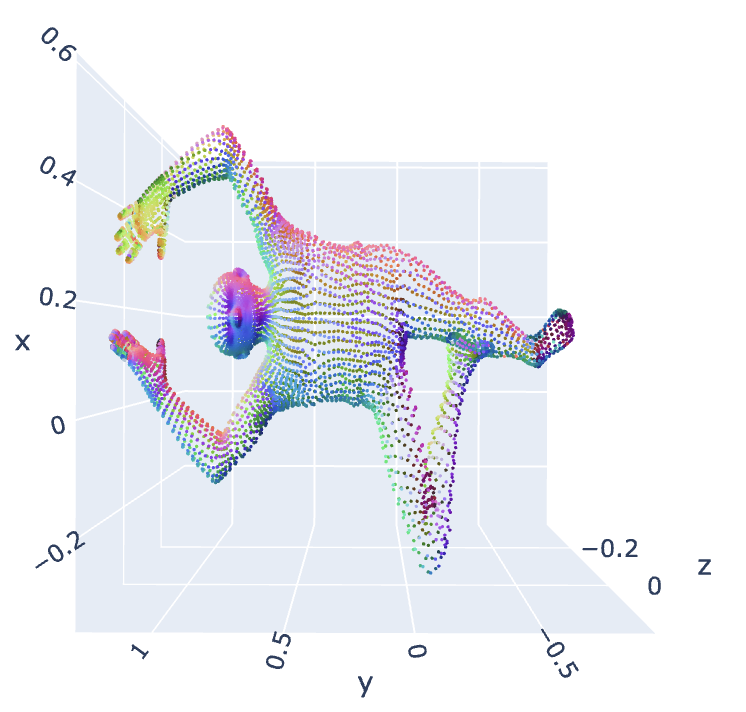
\includegraphics[width=0.9\linewidth, height=0.6\linewidth, keepaspectratio=false]{../Media/example/registration.png}
      \captionof{figure}{Registration cloud}

    \column{0.4\textwidth}
      \centering
      \hspace{1em}
      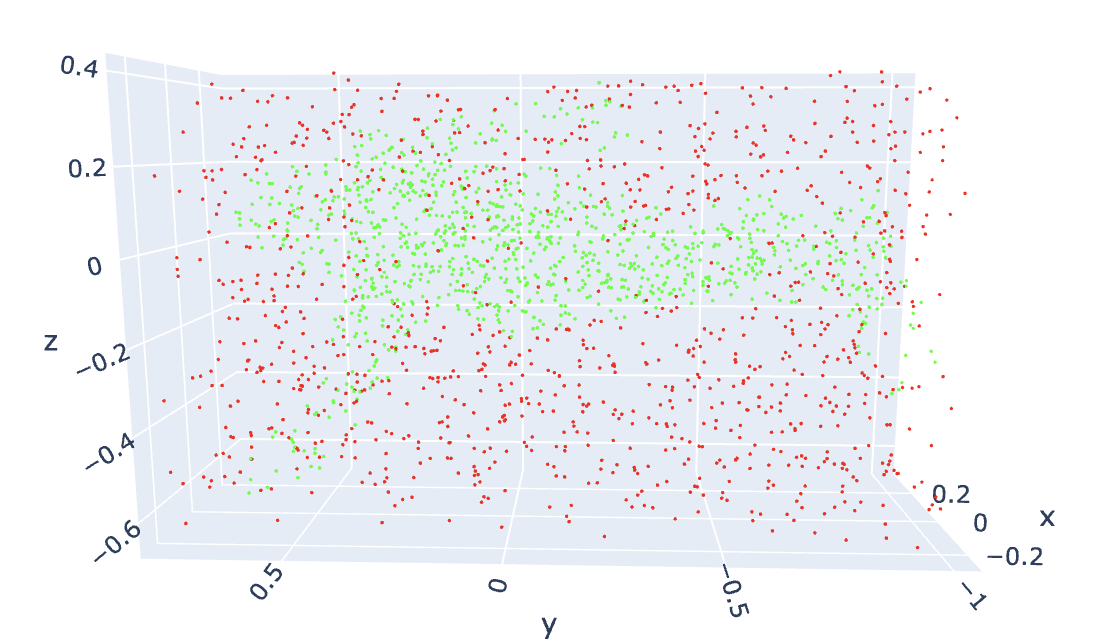
\includegraphics[width=0.84\linewidth]{../Media/example/augmented_noisy_cloud.png}
      \captionof{figure}{Augmented cloud}
  \end{columns}
  
  \end{frame}

\begin{frame}{Label Generation}
  \begin{columns}[T]
    \column{0.45\textwidth}
      For each Sampled Cloud, labels have been generated with the following procedure:
      \begin{itemize}
        \item Measure the distance between the original mesh and the sampled points
        \item If the distance is positive then the point are inside the mesh
        \item If the distance is $0$ the points are on the surface
        \item If the distance is negative outside a small threshold I am considering them outside
      \end{itemize}
  
    \column{0.45\textwidth}
      \vspace{-2em}
      \centering
      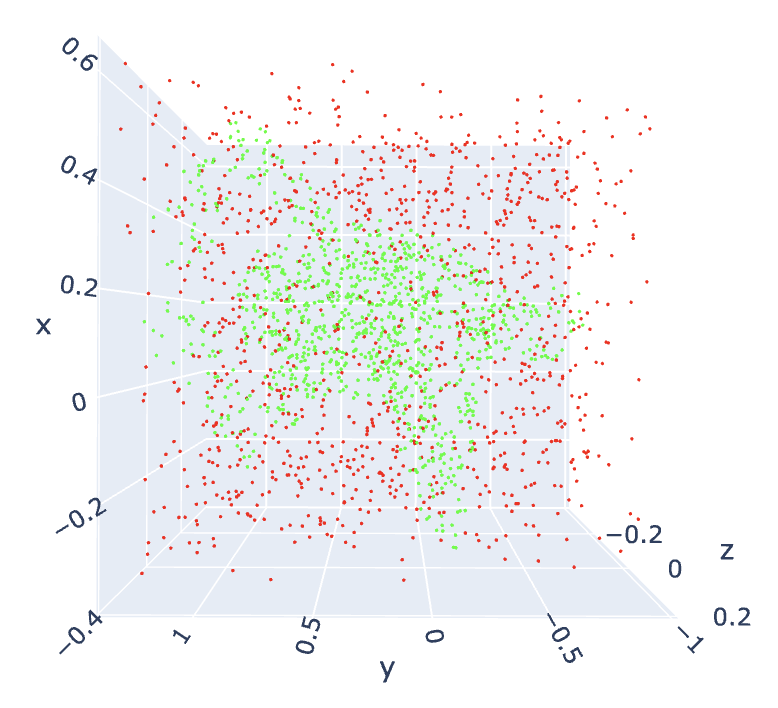
\includegraphics[width=0.9\linewidth]{../Media/example/sampled_cloud.png}
      \captionof{figure}{Example of the Sampled cloud, where with green we represent occupied points and with red the unoccupied ones}
  \end{columns}
\end{frame}

\section{Architecture}

\begin{frame}{Architecture design}
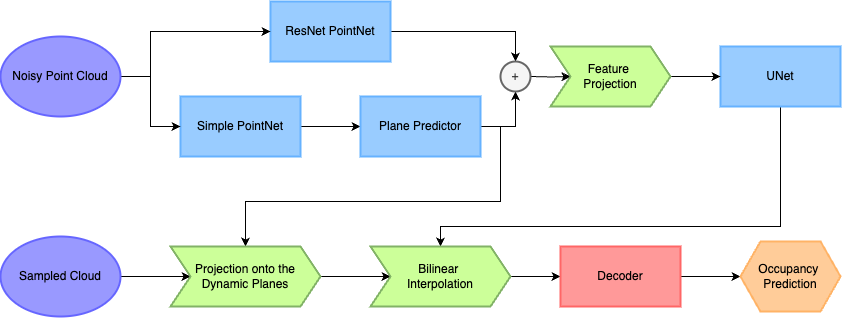
\includegraphics[width=\textwidth]{../media/structure/pipeline_chiaro.png}
\end{frame}

\begin{frame}{Encoder}
The Encoding part takes in input the Noisy Cloud and it's composed by the following steps:
  \begin{itemize}
    \item ResNet PointNet
    \item Simple PointNet + Plane Predictor 
    \item Feature summation + projection 
    \item UNet
  \end{itemize}
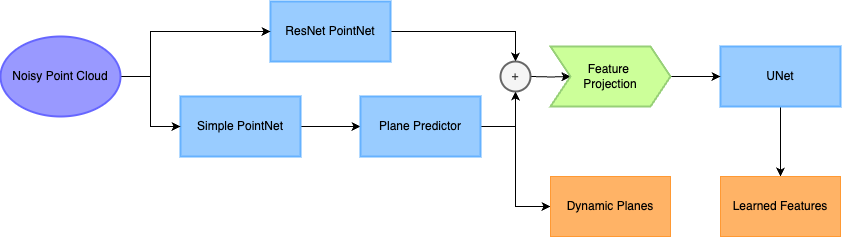
\includegraphics[width=\textwidth]{../media/structure/encoder_pipeline.png}
\end{frame}

\begin{frame}{Decoder}
The Decoding part is composed by:
\begin{itemize}
\item Feature Projection and Bilinear Interpolation
\item Occupancy Network
\end{itemize}
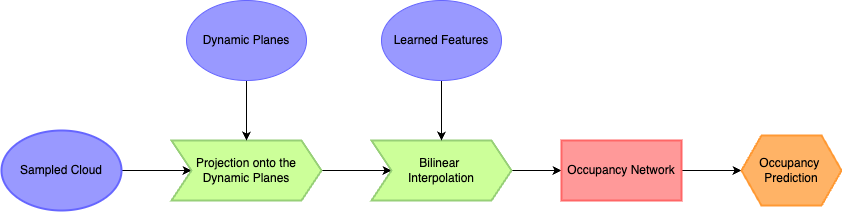
\includegraphics[width=\textwidth]{../media/structure/decoder_pipeline.png}
\end{frame}

\begin{frame}{Projection Operation}
  Both the Encoder and the Decoder have a projection operation involving the features and the \textbf{Dynamic Planes}.
  \begin{columns}[T]
    \column{0.5\textwidth}
      \vspace{1.5em}
      \begin{itemize}
        \item Change of Basis
        \item Orthographic Projection
        \item Normalization
      \end{itemize}
    \column{0.45\textwidth}  
      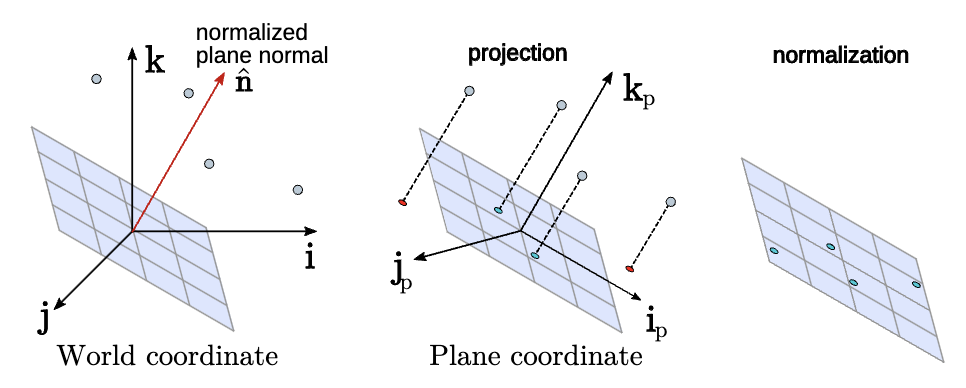
\includegraphics[width=\textwidth]{../media/projection.png}
  \end{columns}
  \vspace{1em}
  \begin{equation}
    \mathbf{R} = \mathbb{I} + [v]_{\times} + [v]_{\times}^2 \frac{1 - k \cdot \hat{\textbf{n}}}{|| v ||^2}
  \end{equation}
  Where $v = k \times \hat{\textbf{n}} $ and $[v]_{\times}$ it's the skew symmetric matrix of the vector $v \in \mathbb{R}^3$.
\end{frame}

\begin{frame}{Bilinear Interpolation}
  \begin{columns}[T]
    \column{0.5\textwidth}
    \vspace{1em}
    \begin{itemize}
      \item \textbf{Definition:}  
      \begin{itemize}
          \item Bilinear interpolation is a resampling technique used to estimate new pixel values on a 2D grid.
      \end{itemize}

      \item \textbf{Concept:}
      \begin{itemize}
          \item It computes the output value as a weighted average of the four nearest pixel values.
          \item The interpolation is performed first in one direction (e.g., horizontal) and then in the other (vertical).
      \end{itemize}
    \end{itemize}

    \column{0.45\textwidth}
      \vspace{-2.5em}
      \centering
      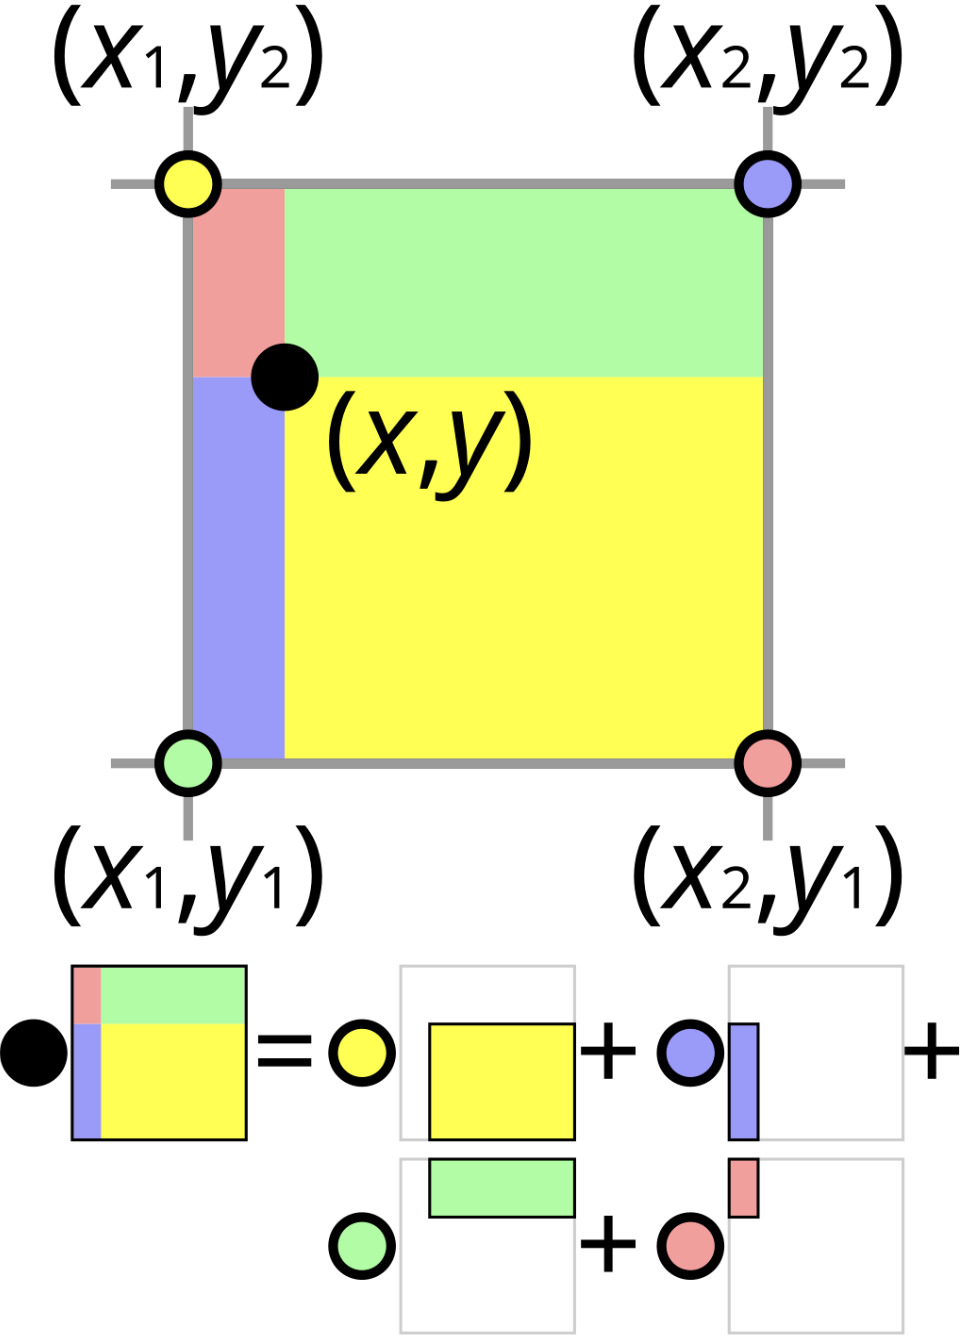
\includegraphics[width=0.65\linewidth]{../Media/bilinear.png}
      \captionof{figure}{Bilinear Interpolation Visualization (credits: Wikipedia)}
  \end{columns}
\end{frame}

\section{Reconstruction}

\begin{frame}{Multiresolution IsoSurface Extraction (MISE)}
    \begin{columns}[T]
      \column{0.5\textwidth}
        \begin{itemize}
            \item Create a grid over all the bounding box 
            \item Evaluate the occupancy of each corner of the voxels
            \item Define the Active voxels as the one composed with at least one occupied corner and one not 
            \item Subdivide each Active voxels into 8 subvoxels ($2x2x2$ grid) and evaluate the new points occupancy
            \item Repeat until the desired resolution is obtained
        \end{itemize}
      \column{0.5\textwidth}
        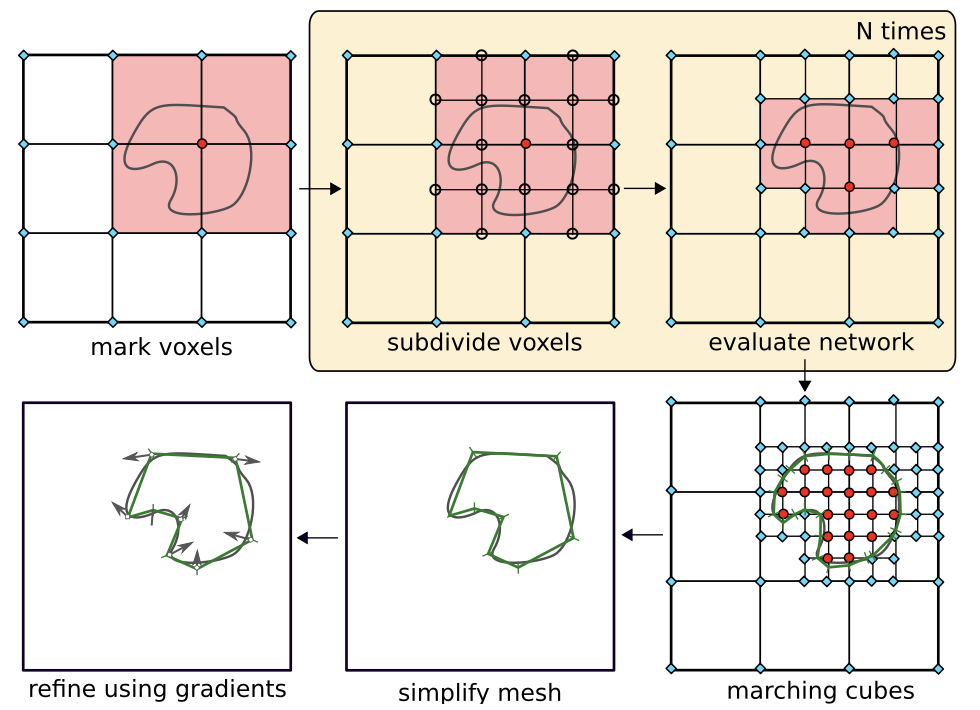
\includegraphics[width=\linewidth]{../Media/structure/mise.png}
    \end{columns}
  \end{frame}

\section{Results}

\begin{frame}{Metrics}
In order to evaluate the performance of our model, the following metrics have been used:
\begin{itemize}
\item Chamfer Distance : \\ 
$
CD(A, B) = \frac{1}{|A|} \sum_{a \in A} \min_{b \in B} \|a - b\|_2^2 + \frac{1}{|B|} \sum_{b \in B} \min_{a \in A} \|b - a\|_2^2
$
\item IOU : 
$ IoU(A', B') = \frac{|A' \cap B'|}{|A' \cup B'|}$
\item F-Score:
\end{itemize}
Add each formula
\end{frame}

\begin{frame}{Loss Performances}
Insert here plots
\end{frame}

\begin{frame}{Metrics Performances}
Insert here just a table with metrics, gpu usage
various types of sampling
\end{frame}

\section{Improvements}

\begin{frame}{Possible Changes and Future Improvements}
\end{frame}

\backmatter
\end{document}